%% gridnets.tex 
%% 2006/05/30 
%% 
\documentclass[conference]{IEEEtran}

\usepackage[dvips]{color}
\usepackage[xdvi]{graphicx}
\usepackage{subfigure}

% correct bad hyphenation here 
\hyphenation{op-tical net-works semi-conduc-tor IEEEtran ESnet OSCARS}

\begin{document}

% paper title
\title{Intra and Interdomain Circuit Provisioning using the OSCARS Reservation System}

% 
\author{\authorblockN{Chin~Guok\authorrefmark{1},
David~Robertson\authorrefmark{1}\authorrefmark{2},
Mary~Thompson\authorrefmark{2},
Jason~Lee\authorrefmark{2},
Brian~Tierney\authorrefmark{2} and
William~Johnston\authorrefmark{1}\authorrefmark{2}}
\authorblockA{\authorrefmark{1}Energy Sciences Network\\
Berkeley, California 94720}
\authorblockA{\authorrefmark{2}Ernest Orlando Lawrence Berkeley National Laboratory\\
Berkeley, CA  94720}}

% make the title area
\maketitle

\begin{abstract}
With the advent of service sensitive applications such as remote controlled 
experiments, time constrained massive data transfers, and video-conferencing,
it has become apparent that there is a need for the setup of dynamically 
provisioned, quality of service enabled virtual circuits.
The ESnet On-Demand Secure Circuits and Advance Reservation System (OSCARS) is 
a prototype service enabling advance reservation of guaranteed bandwidth 
secure virtual circuits.

OSCARS operates within the Energy Sciences Network (ESnet), and has
provisions for interoperation with other network domains.
ESnet is a high-speed network serving thousands 
of Department of Energy scientists and collaborators worldwide.

OSCARS utilizes the Web services model and standards to implement communication
with the system and between domains, and for authentication, authorization,
and auditing (AAA).  The management and operation of end-to-end virtual 
circuits within the network is done at the layer 3 network level.  
Multi-Protocol Label Switching (MPLS) and the Resource Reservation Protocol 
(RSVP)
are used to create the virtual circuits or Label Switched Paths (LSP's). 
Quality of Service (QoS) is used to provide bandwidth guarantees.

This paper describes our experience in implementing OSCARS, collaborations
with other bandwidth-reservation projects, including interdomain testing, and 
future work to be done.

\end{abstract}

% no keywords
%\begin{keywords}
%Multi-Protocol Label Switching (MPLS); Resource Reservation Protocol (RSVP); Quality of Service (QoS);
%ESnet On-Demand Secure Circuits and Advance Reservation System (OSCARS)


% for peerreview papers, inserts a page break and creates the second title.
% Will be ignored for other modes.
\IEEEpeerreviewmaketitle

\section{Introduction}
Large-scale science is increasingly important as attention turns to the
study of the most complex, subtle, and elusive natural phenomena.  Such
study is completely dependent on world-wide collaborations of scientists
and widely dispersed resources such as computing, data, and instruments.

Over the past several years significant improvements have been made in the
computing and communications infrastructure necessary for support of these
collaborations.  Network bandwidths have increased, data transport protocols
have improved, and security issues have become better understood.  However,
for the network to fully enable such distributed science, network
communication must be delivered as a manageable service to the distributed
applications just as computing is.
 
The goal of OSCARS is to manage and schedule high-impact network services
associated with these collaborations.  These services, which move 
multi-terabyte to multi-petabyte datasets from experiments and simulations,
and may include high-end remote visualizations, cannot be provided 
cost-effectively by best-effort service on a production network.  In this context, services must 
be \emph{deterministic}, implying a defined and guaranteed service level.
At a minimum, bandwidth must be guaranteed. Other possible future service guarantees
include loss rates, latency, and jitter.

There are significant challenges to allowing users to schedule high-performance 
network service on a production network. Some of these challenges are: allowing 
only authorized users to create and manage high-performance services;
providing an easy-to-use interface for scheduling and managing network 
resources; limiting the impact of high-performance traffic on other network
traffic; 
coordinating quality of service end-to-end 
across more than one autonomous network domain;
and handling changes in network paths between the time a reservation is
scheduled and when it is claimed.  OSCARS currently addresses all but the
last item, where work is still in progress.

Due to the highly distributed nature of large scale science,
the service framework for OSCARS is being
developed in coordination with other community network provisioning efforts. 
The closest coordination is with the Internet2 BRUW \cite{bruw}\cite{riddle} system. 
A version of BRUW was used as the starting point for OSCARS, and now the two 
projects share a common code base. Interoperability testing is on-going with 
Internet2 sites. 

OSCARS has been deployed within ESnet,
which is a nation-wide network that serves approximately 42 directly connected 
sites around the country.  Internally, ESnet manages about 270 routers and 
systems throughout the network and its operations centers.  The current ESnet 
architecture is that of a high-bandwidth (10/2.5 Gb/s) backbone ring 
around the country, with hubs at strategic locations.  The sites, which are 
mainly
large Office of Science laboratories, are connected to the hubs via metro rings at 2 x 10Gb/s speeds.
OSCARS faces the constraint of operation within this production 
network, where 99.9+\% reliability is critical.

Having the ability to dynamically allocate capacity in the network exclusively 
to a scheduled service, to the exclusion of normal priority traffic, introduces 
risks.
Throughout the design and implementation of OSCARS, security aspects were
paramount.  The impact of an abuse could be very
large.  A DoS attack could prevent reservations from being processed.  If the
service is compromised, an attacker could disable the wide area network.

This paper describes how OSCARS addresses the above constraints and
risks while implementing a scheduling system.  Section II covers the 
OSCARS architecture, and Section III describes the details of
path setup and reservation handling. Section IV outlines some issues with cross-domain
interoperability, and covers other reservation systems and 
collaborative efforts, as well as 
an example of an interoperability test between OSCARS and BRUW.
Section V covers security, including system, interdomain, and authentication,
authorization and auditing issues.
The final section touches briefly on the future work that needs to be performed
to handle a dynamically changing network (which may invalidate existing
reservations), and to set up end-to-end circuits between domains
in a secure, standards-based fashion.

\section{Architecture}

The intent of OSCARS is to create a service for dynamic QoS path establishment
that is simple for users to use, and easy to administer.  The only task 
required of a user is to make a bandwidth reservation.  Reservation can be made 
either for immediate use or in advance for either one-time use or persistent use, 
e.g. for the same time everyday. The user does not have 
to configure an alternate routing path, nor mark the packets in any way.  All 
necessary mechanisms needed to provide the user with a guaranteed bandwidth 
path are coordinated by a  \emph{Reservation Manager} (\textbf{RM}) and 
managed by the routers in the network.

\begin{figure}
 \centering 
   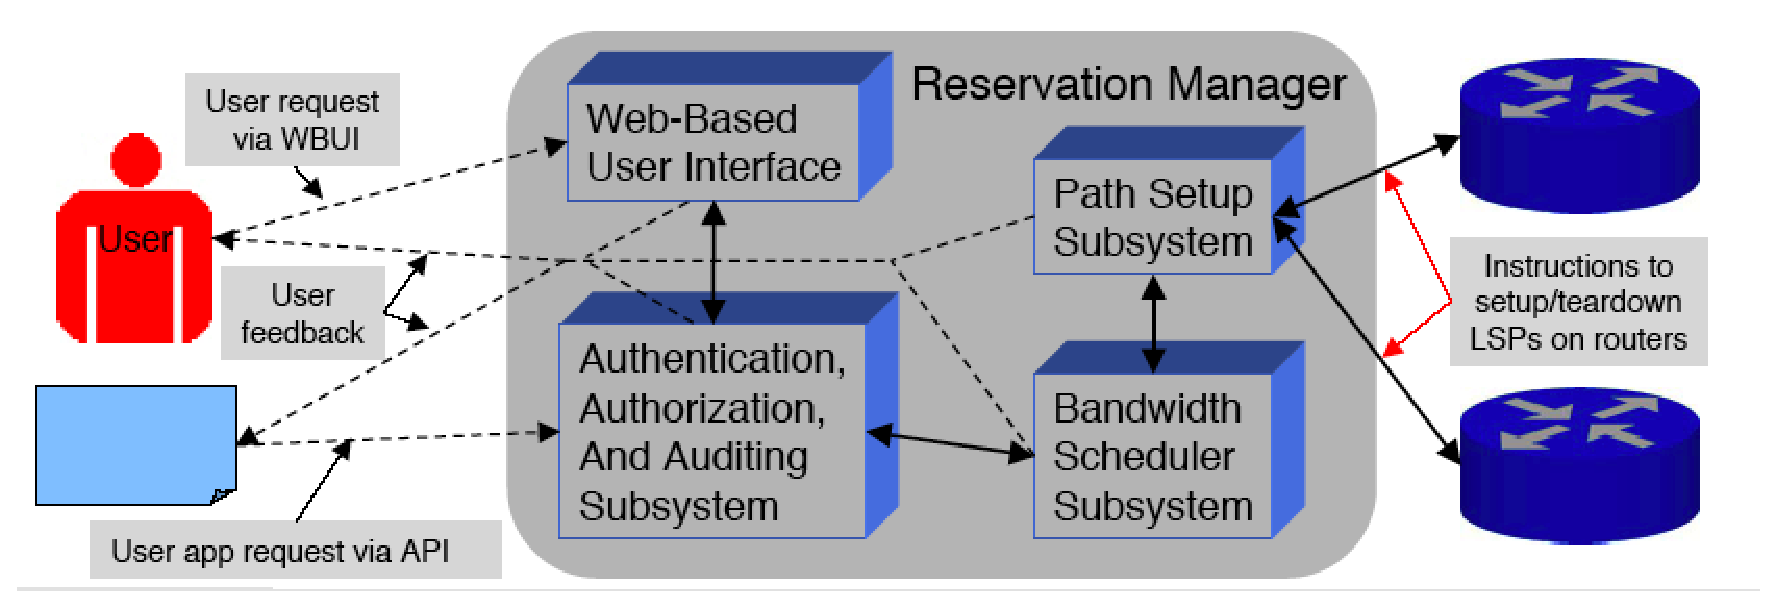
\includegraphics[scale=0.3]{pict1.eps}
   \caption{OSCARS Architecture.}
 \label{fig:oscars_arch}
\end{figure}

\subsection{Components}

The RM is comprised of three components:  the 
 \emph{Authentication, Authorization, and Auditing Subsystem} (\textbf{AAAS}), 
the  \emph{Bandwidth Scheduler Subsystem} (\textbf{BSS}), and the  \emph{Path 
Setup Subsystem} (\textbf{PSS}) (Figure 1). All persistent information is 
stored in a database.  
The RM provides simple Web forms for creating and managing reservations, 
setting authorization policy and other administrative tasks (the Web-based
user interface in the figure).
It also supports a SOAP message interface API to support programmable 
reservation management and requests from other network service providers.

The AAAS is responsible for authenticating and authorizing all external 
requests, for logging request information, and sending notifications to
users and administrators of the results of calls made to the RM.  It also
handles a number of internal requests related to management of users 
and resources.

The BSS is responsible for scheduling reservations.  It handles
requests to schedule bandwidth reservations, list reservation details,
modify and/or cancel one or more existing reservations, and provide a summary
of all current reservations.

To perform these functions, the BSS keeps information about past,
pending, and current reservations, and tracks the current topology and state of
the network.  As part of scheduling a reservation request, the BSS must
determine whether the requested bandwidth will over-subscribe any of the links
in the path to be set up within the network.

The PSS is responsible for setting up and tearing down the on-demand bandwidth 
paths. This is accomplished by making the necessary configuration changes in 
the routers to create or destroy a \emph{Label Switched Path }(\textbf{LSP}) at the time
indicated by the BSS. The authentication and authorization method for the PSS 
is internal to the ESnet network and is specific to the router platform 
(currently Juniper or Cisco) being configured.  It is therefore distinct from 
the AAAS used by the BSS.

\subsection{Implementation}

Web services standards are used wherever possible.  SOAP \cite{SOAP} messages are
used for communications between clients and the RM, and 
the \emph{Web Services Definition Language} (\textbf{WSDL}) \cite{WSDL} is used for the service description.
 
The resource manager is implemented as an Apache Web server configured for
mod\_perl, a SOAP server, two databases within a MySQL server, and a set of 
Perl packages that implement the AAAS, BSS, and PSS.  The Web server is
used to accept CGI requests, and to forward API requests directly to the SOAP 
server.  CGI requests are reformatted as SOAP requests, and then forwarded to 
the SOAP server.  One database contains persistent information related to
reservations and AAA, and the other contains a representation of the local
network topology.  Security issues are discussed in the section on security
below.

\section{Paths and Reservations}

\subsection{Path Setup}

The procedure of a typical path setup is as follows:

\begin{enumerate}
\item
A user submits a request to the RM (using either an API or
an optional Web front-end) to schedule an end-to-end path (e.g. between an
experiment and computing cluster) specifying start and end times, bandwidth
requirements, the source host that will be used 
to provide an application access to the path, and the destination host.

\item
This information is stored by the BSS in a database, and a script 
periodically checks to see if the PSS needs to be contacted, either to create 
or tear down the circuit.

\item
At the requested start time, the PSS configures the 
ESnet \emph{provider edge} (\textbf{PE}) router
(at the start end of the path) to create an LSP with the
specified bandwidth.

\item
Each router along the route receives the path setup request 
via \emph{Reservation Resource Protocol} (\textbf{RSVP}) \cite{rfc2205}
and commits bandwidth (if available) creating an end-to-end LSP.  The RM is
notified by RSVP if the end-to-end path cannot be established.

\item
Packets from the source (e.g. experiment) are routed through the site's
LAN production path to ESnet's PE router.  On entering the PE router,
these packets are identified and filtered using flow specification parameters
(e.g. source/destination IP address/port numbers) and policed at the specified
bandwidth.  The packets are then injected into the LSP and switched (using MPLS)
through the network to its destination (e.g. computing cluster).

\item
A notification of the success or failure of LSP setup is 
passed back to the RM so that the user can be notified and the event 
logged for auditing purposes.

\item
At the requested end time, the PSS tears down the LSP.
\end{enumerate}

\subsection{Path Discovery}
There are two scenarios for creating a path in OSCARS.  One is where the
reservation request does not contain any connectivity information outside of
the source and destination (IP addresses).  The other is where a request
contains additional routing information such as the ingress and/or egress 
PE routers within the OSCARS administrative domain.

In the scenario where an ingress PE router is not explicitly communicated, 
OSCARS does a traceroute (from the core of the network) towards the source IP 
address of the traffic. As the traceroute
progresses, each router in the trace is checked to verify if 
it is within the administrative control of OSCARS. As soon as OSCARS 
encounters a router that
is outside of its administrative domain, OSCARS marks the last router (within 
its administrative control) as the ingress PE router.

In the scenario where the egress PE router is not contained in the reservation 
request, 
the destination IP address is used as the target of the traceroute (sourced 
from the ingress PE router).
Using the same method outlined in the previous paragraph, the egress PE router 
can be determined.

With the ingress and egress PE routers identified, the path (or route) between 
the two can be trivially determined.

The need for OSCARS to support reservations with explicit ingress and egress PE
routers is to
facilitate traffic engineering for sites or networks that have more then one 
peering connection with ESnet.

In the event that the virtual circuit extends beyond OSCARS' administrative 
domain,
routing information harvested from the \emph{Border Gateway Protocol} 
(\textbf{BGP}) on the egress PE router is used to determine the next
\emph{Autonomous System} (\textbf{AS}) that the request should be forwarded 
to.   The AS number is
checked against a list of known administrative domains that have reservation 
systems
that are cooperating with OSCARS.  If a match is found, the request is 
forwarded to the downstream AS.

\subsection{Advanced Reservations }
In OSCARS, advance reservations are handled in a slot based manner. This equates
to 'first come first served' for bandwidth across any particular link at any
moment. As each reservation is requested in OSCARS, the end-to-end path is
computed for that reservation. Once the entire path though all the routers
controlled by OSCARS has been computed, each link in the path is checked for
available bandwidth. To check the bandwidth of a link, all outstanding
reservations for that link during the time of the proposed reservation are
queried from the data base. Then all the reserved bandwidth amounts are
calculated and compared to the actual capacity of the link. If the requested
amount of bandwidth plus all outstanding reservations is more then the allocated
amount of bandwidth available for reservations on that link (in this case
50\%), then the reservation fails. Only if there is enough bandwidth 
available on all links is the reservation committed into the reservation system.

In the future, in the case where the capacity of a link changes (e.g. a link 
upgrade or failure), all outstanding reservations
that involve the use of that link will be queried from the system and 
recomputed.
This will be done to ensure that there is adequate bandwidth available on the
link when it comes time to provision the reservation.

\subsection{Provisioning and Policing}
To facilitate bandwidth guarantees, provisioning and policing are needed to 
enforce reservation and usage limits.  In OSCARS, RSVP is used as the 
provisioning mechanism.  To ensure that resources are not over-subscribed, QoS 
is carefully configured to provision queues within the network core.  Within 
ESnet, traffic utilizing the OSCARS service is classified into a 
Class-of-Service distinct from all other traffic and isolated into a separate 
queue by 
itself.  The size of this queue is configured to match the RSVP bandwidth 
limits on each interface, e.g. if the RSVP bandwidth limit on an interface is 
50\%, the OSCARS queue is also set at 50\%.  This ensures that the RSVP 
provisioned bandwidth will translate to available network bandwidth within 
the network core.

With all of OSCARS traffic using the same Class-of-Service queue within the 
network core, it is vital to ensure that the bandwidth usage of each individual 
RSVP reservation is strictly adhered to.  This prevents the aggregate traffic 
from overrunning the queue dedicated to the OSCARS service.  To do this, each 
flow utilizing the OSCARS service is policed individually according to the 
reservation bandwidth request.  This policing is done at the ingress point to 
ESnet.


\section{Interdomain Reservations}

Guaranteed bandwidth paths are most effective 
when the reservation spans end-to-end.  This however, introduces the 
complexity of extending virtual circuits beyond the scope of a 
single administrative domain to multiple domains.  To facilitate this, 
neighboring domains must agree on several levels, mainly, the management plane, 
control plane, and data plane:

\begin{itemize}
\item
The management plane dictates policies and procedures for authentication, 
authorization, and usage.  This essentially amounts to a \emph{Service Level 
Agreement} (\textbf{SLA}) between peer networks.  In almost all cases, the 
usage 
condition outlined within an SLA determines the maximum aggregate limit.  
This implies that individual bandwidth requests are managed by the reservation 
system of the originating AS and not propagated independently to the transit 
AS's 
(i.e. the transit AS will see the request as coming from the originating AS and not the individual making the request).

\item
The control plane dictates the way control messages, such as setup and 
teardown requests, are exchanged between the networks, e.g. RSVP signaling.
At this point in time, interdomain interoperability efforts do not permit
the end-to-end signaling of LSP's via the control plane (i.e. interdomain 
exchange of RSVP messages).  This is because
there is no vendor implementation that can enforce complex SLA requirements of 
the various administrative domains.  As such, end-to-end virtual circuits are
comprised
of intradomain LSP's stitched together at agreed interconnection points.

\item
The data plane handles how user traffic is forwarded from one network to 
another network, e.g. IP packets, Ethernet VLAN packets, etc.  This is one of 
the fundamental issues that must be resolved in order for an interdomain 
end-to-end virtual circuit to be successful.  Complications arise when 
peering RM's provision virtual circuits at different network layers (e.g. 
GMPLS LSP, MPLS LSP).  The solution to bridging the data planes is part of 
ongoing collaborative efforts.
\end{itemize}


\subsection{Related Work}

There are several implementations of network resource management and
service provisioning systems in existence today.  These include the DOE funded
TeraPaths \cite{terapaths} and UltraScience Net \cite{usn} projects, the NSF funded CHEETAH \cite{veeraraghavan} and
DRAGON \cite{yang}\cite{dragon} projects,
Internet2's BRUW \cite{bruw} and HOPI \cite{hopi} projects, CANARIE's UCLP \cite{canarie} 
project, and GEANT's
BoD (GN2-JRA3) \cite{geant} and AMPS (SA3) \cite{geant-amps} activities.

All of these projects, as well as OSCARS, are based on a Web services 
interface to reserve and configure a path across the network. However, they 
have slightly different ways of handling reservations and AAA issues.

Dragon uses OSPF-TE \cite{ospf-te} for intradomain routing, and a component called
the Network Aware Resource Broker (NARB) for interdomain routing.
Dragon plans to use the Common Open Policy Service (COPS) \cite{cops}
protocol for support of policy provisioning (COPS-PR) \cite{cops-pr}.

Canarie, Canada's advanced Internet development organization, has been
working on a project called User Controlled LightPath (UCLP).  UCLP
allows end-users to create their own static independent IP network as a subset
of a larger optical network and to have total control over their share
of network.

The University of Amsterdam's Advanced Internet Research group has
published a number of papers
describing both the networking and the AAA issues for such a system,
including \cite{gommans05} \cite{gommans06} \cite{demchenko} . 
They are using the IETF AAA Framework
\cite{rfc2904}, and use XACML \cite{XACML} to describe policy. They have also defined a
\emph{Network Description Language} (NDL), which is a RDF-based method to
describe networks, to facilitate interdomain interoperability \cite{ndl}.

In the OSCARS, BRUW, TeraPaths, and AMPS projects, IP connectivity (layer
3) is used as the data plane exchange.  This facilitates interoperability
trials with no additional network connection needed outside of the production
peering exchange.

It should be noted that OSCARS and BRUW now share a common code base, but
are configured differently due to differing methods of network administration
and user authentication.

The other projects mentioned use the optical network layer (i.e. layer 1), 
creating lightpaths.  The last section of this paper points out the
necessity of future work to bridge projects using different layers.

\begin{figure}
 \centering 
%   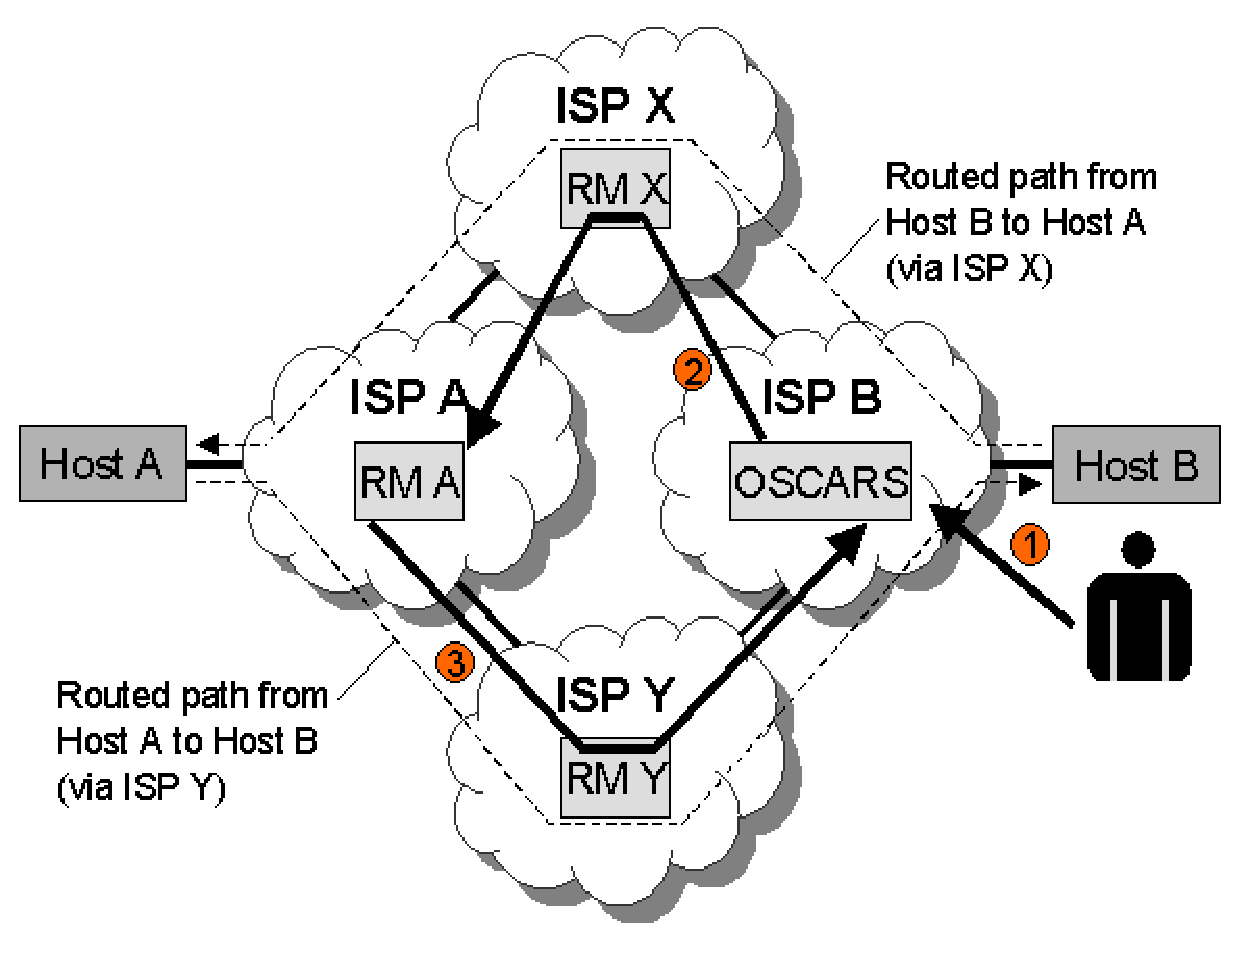
\includegraphics[scale=0.40]{pict2.eps}
   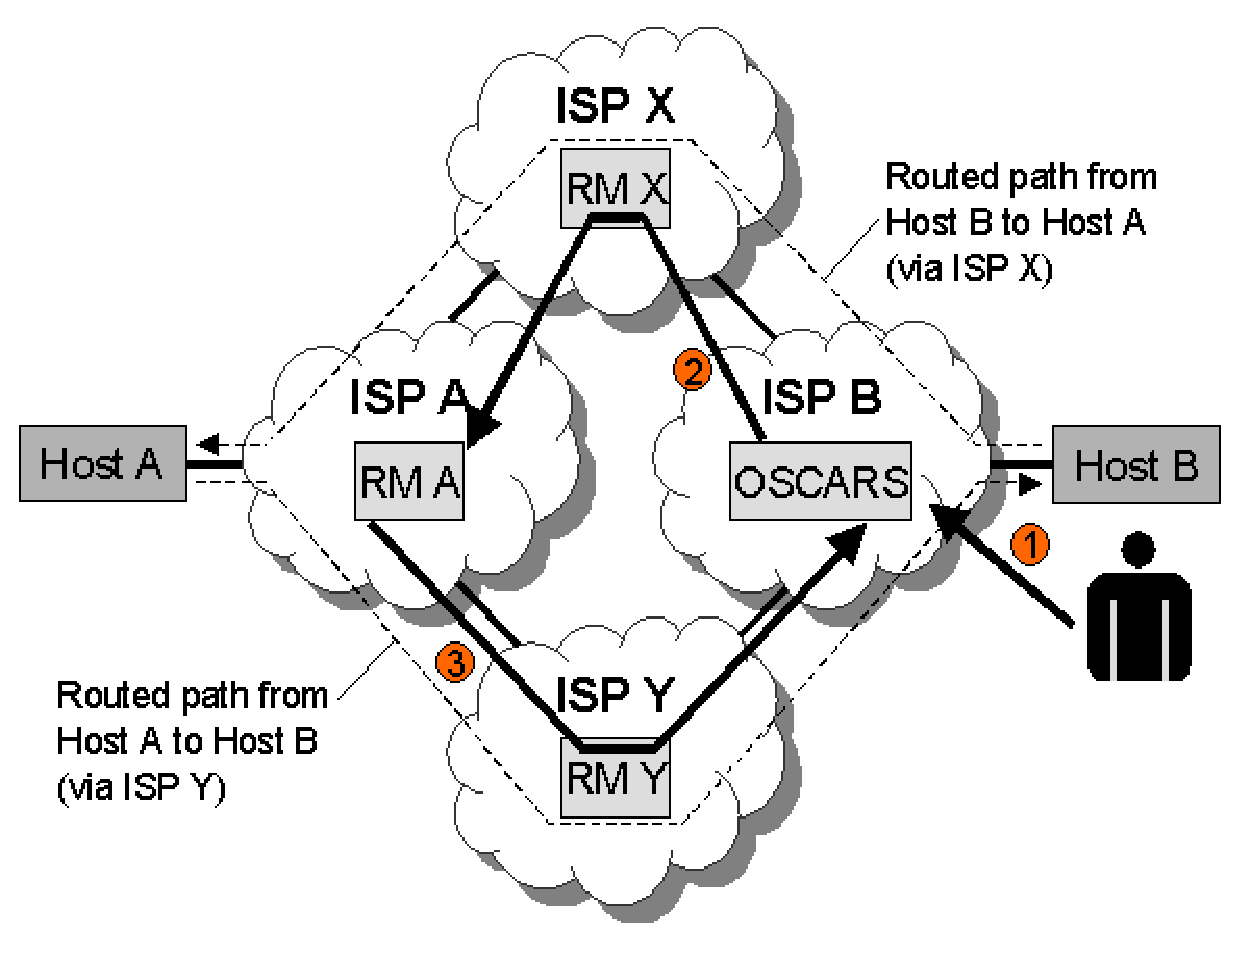
\includegraphics[width=3in]{pict2.eps}
   \caption{Interdomain Path Setup.}
 \label{fig:interdomain_path_setup}
\end{figure}

\subsection{Interdomain Path Setup }
One of the more complex examples of using the OSCARS reservation system
involves the setting up of a virtual circuit between two hosts that span
several administrative domains.  For example, imagine setting up a
virtual circuit between Host A and Host B, where Host A is controlled by a
remote reservation system RM A in ISP A, and Host B is part of the local
OSCARS reservation system in ISP B (see Figure 2). The routed path from ISP B
to ISP A transits ISP X, but the reverse path from ISP A to ISP B is via ISP Y.
In order for an OSCARS' user to make an interdomain virtual circuit reservation
request from Host A to Host B, the following must occur.
\begin{enumerate}
\item 
On receiving the request from the user, OSCARS
computes the virtual circuit path and determines the downstream AS (ISP X).
\item
A \emph{Forward Create} message is sent across the network (ISP X) towards Host
A, crossing all intervening reservations systems (RM X), until it reaches the
last reservation system (RM A) that has administrative control over the network
(ISP A) that Host A is attached to.
\item
The remote reservation system (RM A) then computes the path of the virtual
circuit, and initiates the bandwidth reservation requests from Host A towards
Host B (via ISP Y).  This can be especially complex when the path back (from
Host B to A) is asymmetric and traverses AS's (e.g. ISP Y) that were not
traversed on the forward path, causing the local OSCARS to see the path
originating from a different AS than it originally sent the \emph{Create} request
out to.

\end{enumerate}


To facilitate interdomain virtual circuit setup, a WSI-BP \cite{ballinger} compliant WSDL   specification for the 
network-network interface has been specified following the model of 
GEANT's Advance Multi-domain Provisioning
System (AMPS)  \cite{geant-amps} . This interface is being tested with the 
TeraPaths \cite{bradley} project. 
Having a WSDL specification allows reservation systems to communicate with one 
another in a well defined 
syntax. While the OSCARS interface is similar to the one specified by AMPS, these
are both quite different from the TeraPaths interdomain WSDL.
One of the next challenges in
automating trans-domain circuit setup is to define a standard request for interdomain
reservations. It would then be up to the individual reservation system to 
transform the standardized messages to internal calls to reserve and provision the 
virtual circuit.

 \subsection{Interoperability Tests}

In April 2006, an interdomain guaranteed bandwidth path between Abilene and 
ESnet was dynamically negotiated and configured by the BRUW and OSCARS systems 
respectively. The unidirectional 25Mb/s guaranteed bandwidth path was 
configured between an Internet2 test host in Indianapolis, IN and an ESnet 
Performance Center \cite{esnet-pc} host in Sunnyvale, CA.  The path consisted of two 
unidirectional MPLS Label Switched Paths (LSP's), one in Abilene, and the 
other in ESnet, \emph{stitched} together at the Abilene-ESnet peering point in 
Chicago, IL.

% example table
\begin{table}
 \centering
 {\scriptsize
 \begin{tabular}{|c|c|c|c|}
 \hline
 Test     & Test       & Guaranteed & Throughput  \\ 
 Protocol & Parameters & Bandwidth  & Achieved    \\ \hline \hline 
 UDP      & Throughput  & No         &   30Mb/s   \\ \cline{3-4}
          & Set: 30Mb/s& Yes (25Mb/s)&   24.6Mb/s \\ \hline
 TCP      & TCP Window & No         & 158.0 Mb/s  \\ \cline{3-4}
          & Size: 1MB  & Yes (25Mb/s)&  14.7Mb/s  \\ 
          & Latency: ~50 ms &          &            \\  \hline
 \end{tabular}
 }
 \caption{IPerf results of guaranteed bandwidth paths.}
 \label{tab:bandwidth}
\end{table}


Bandwidth tests using IPerf \cite{iperf} (see Table ~\ref{tab:bandwidth}) revealed
predictable results except for the guaranteed bandwidth TCP transfer.

The guaranteed bandwidth (25Mb/s) TCP transfer should have yielded a 
throughput closer to 25Mb/s.  On further investigation, it was determined 
that the 
discrepancy between the policing bandwidth and the achieved bandwidth was 
likely the result of two things, first, the lack of traffic shaping at the 
source end, and second, Juniper's policing function.  Similar results have 
been documented by others \cite{martelli}.


\section{Security}
Since OSCARS is being deployed on the ESnet production network, security was 
an absolute requirement from the beginning. Good security needs mechanisms that are easy to understand, install, use, and administer. It is very important that there
are no unintended consequences of authorization policy decisions.

The following section details steps taken to secure the machines and 
servers running OSCARS, and the remaining security sections cover AAA.

\subsection{System}

An Apache2 Web server on an open ESnet machine is used to forward all 
requests to the RM Web server, which runs on a machine behind a firewall. 
This forwarding process is transparent to the end user, and hides the location 
of the internal server.

The internal Web server only accepts https connections from the open machine.
The RM SOAP server only accepts requests from the Web server on the internal 
machine
or digitally signed SOAP messages encapsulated in https messages forwarded from the open Web server.
Database server processes run as an unprivileged user without a login 
shell.  The database server only accepts requests from the SOAP server.


\subsection{Authentication}
OSCARS authenticates the sender of all requests that it receives.
The Web based interface and the SOAP server API use the
authentication mechanism that is most natural for them. The Web server
requires a username and password for authentication on the first
access during which it creates session information for the user and a
8-hour cookie referencing this information. This cookie is used on subsequent
connections. All communication with the Web server takes place over
encrypted https in order to protect against the stealing of passwords
or cookies. The SOAP API distinguishes between requests coming from
the Web server on the local host, which it assumes have been authenticated
as just described, and requests coming from the open Web server. The 
latter requests  must be digitally signed messages \cite{eastlake} signed by the
originator of the message. The AAAS verifies the signature and the signing 
certificate to authenticate
the user. It then uses the subject name from the signing certificate
to identify the user. Because there is a Web server on the open network 
interposed between the
requester and the SOAP server behind the firewall, digitally signed messages 
are 
needed to do end-to-end client authentication and to support proxy certificates
as a single-signon mechanism. Both the username/password and certificate 
authentication methods use the database user table to
determine if the request is coming from a legitimate user. This table
contains a mapping of the OSCARS user name, password, subject name
from the certificate and the certificate itself, as well as other
information about the user.

Requests for or about interdomain
reservations are authenticated in the originating domain on the basis
of an individual user, and in the subsequent domains on the basis of
the RM in the adjacent domain.  This approach follows the AAA  Authorization
model defined by the IETF Networking Group. \cite{rfc2904}. In this model
users are authenticated and authorized for actions in their home domain and 
interdomain authorization depends on SLA's between domains (AS's) and the
assurance that  a request is coming from a trusted server in a trusted domain. Normally all requests between domains will be a SOAP \emph{forward}  message
signed by the RM. The OSCARS RM has a list of the
cooperating RM certificates as well as a list of
permissions for those AS's. In effect a service level agreement gets
implemented in the user and authorization tables in the database. The forward
message includes the name of the originating user, in case other
domains wish to use that information for authorization or auditing.
Currently, at the time of provisioning no further authentication is
done. Provisioning is triggered by the time of the reservation. Once
the provisioning has been completed, any traffic coming from the
specified ingress router is able to use the higher class of bandwidth.

\subsection{Authorization}
Once a request has been authenticated as from a registered OSCARS
user, that user's authorization is checked against an authorization
table in the database. This implementation was inspired by one
author's experience with the ROAM authorization service of the
FusionGrid \cite{burruss}. This approach allows the use of standard database
commands to define resources and permissions and to manage and check
authorizations. As long as there are not too many resources,
permissions or users, it provides an easily managed and understood
access control scheme. While there are many "policy languages" 
(e.g. S-expressions,
SAML, XACML) that facilitate the expression of complex access policy, they
typically require the use of a parsing engine and interpreter to evaluate a 
request for action. If the administrators start specifying complex policy, it
becomes difficult to tell at a glance exactly what access is allowed. With the simple database 
policy, it is easy to query exactly who has access to a resource and what
resources a particular user or AS  has. Thus an ESnet system administrator who is
not directly part of the OSCARS implementation team could check on (or modify)
who had rights to make reservations or control routing on "his" network. 

In the case of OSCARS,  access is controlled for 
the management of reservations, users and domains. The permissions that can
be granted are view, manage (modify), maximum-bandwidth for a
reservation, duration of a reservation and the right to specify
routing.  The maximum number of authorized users at any one time is estimated 
to be around 50, remembering that OSCARS only needs to know
about users at ESnet sites who have the rights to schedule
high-bandwidth service and cooperating RM's in other
domains. If the number of users grows beyond this point, the tables can be
expanded to define groups (e.g. roles or projects) of users.

\subsection{Auditing}
At this point, the OSCARS server logs all significant activity such as
creating or canceling reservations. In addition a list of all
reservations is kept and can be read with the \emph{list reservations}
operation. As was mentioned above, in interdomain requests, the name
of the originating user is passed to the next domain where it can be
used for either authorization or auditing.


\section{Conclusions and Future Work}

OSCARS is one example of a system that will become increasingly necessary
as experiments such as the Large Hadron Collider become operational.  It
allows users to easily schedule in advance the 
network bandwidth necessary for their experiment or simulation.  Since it
provides the ability to change router configurations in a production network,
maintaining security is an integral part of its operation.

A number of issues need to be addressed before such systems become
production level in complex network environments where many autonomous
domains may be involved, and where network topologies may be constantly
changing.

\subsection{Topology Changes}

A key consideration, when running OSCARS as a production service, is the ability
to recover from both scheduled and unscheduled network outages or changes.  This
is particularly complex when dealing with bandwidth reservations made for a
future date.  For example, in the event of an unscheduled network outage, future
reservations committed on the affected links must be recalculated. This can be
further complicated if the outage period is unknown.  The converse is also true.
If a new link were to be added or upgraded, increasing the bandwidth allocation
for future reservations creates an inconsistent view with the current state of
the network.  To deal with this, OSCARS
has a polling mechanism that constantly
compares the current state of the network to the state that is reflected in the
OSCARS topology database. If there are differences that affect the
characteristics of a link, the new topology is pushed into the OSCARS database
and all outstanding reservations that use that link are queried from the
database. This is possible since the complete path of all reservations is kept
in the database along with the reservation. Then all the reservations are
recomputed in the order they were placed into the OSCARS system, to ensure that
the requested resources are still available.  In the event that the necessary
resources are unavailable for a reservation that has been entered into OSCARS,
the reservation's state will be changed to \emph{unavailable} and a notice will be
sent to the administrators informing them of the problem.

\subsection{Network-Network Interface}
With the objective of interoperability between the different networks,
comes the need for defining standard interfaces (i.e. Network-to-Network
Interface (NNI)).  This is to facilitate the sharing of network state and
request information in quantifiable characteristics that are common to
collaborating networks.  This could include properties such as connectivity
(topology), bandwidth, latency, and jitter.  There are several documents
that have been published by the different projects as well as organizations
related to this work (e.g.: Geant \cite{geant},  Univ Amsterdam \cite{ndl}, 
Canarie UCLP \cite{canarie-interop}, IETF CCAMP \cite{ietf-ccamp}). However due to the
heterogeneity of network implementations and deployments, generating a single
framework to quantify all networks is challenging.

\subsection{Hybrid Data-Planes}
With the emergence of numerous reservation systems, it is becoming evident 
that there is a need to bridge these systems which provision virtual circuits 
at different network layers.
For example, OSCARS and BRUW provision MPLS LSP's over an IP (layer 3) shared 
network, whereas DRAGON and CHEETAH use
GMPLS to set up lightpaths over a lambda switched (layer 1) network.
The challenge here is to bridge the two systems such
that an end-to-end connection appears to be seamless to the end-user.

In addition, numerous complications arise when reservation systems managing 
disparate data planes attempt to exchange connectivity information.  First, 
there is a need to translate or map connectivity information such that it is 
usable by the reservation system receiving the information (e.g. layer 1 
connectivity information is meaningless to a layer 3 reservation system unless 
it is associated with an IP address).  This is the approach explored by DRAGON.
Second, there needs to be a mechanism to redistribute multi-layer connectivity 
information. Within the IP layer, this is done via BGP.  At lower network 
layers, no such comparable protocols exist.

% Reminder: the "draftcls" or "draftclsnofoot", not "draft", class option
% should be used if it is desired that the figures are to be displayed while
% in draft mode.

% An example of a floating figure using the graphicx package.
% Note that \label must occur AFTER (or within) \caption.
% For figures, \caption should occur after the \includegraphics.
%
%\begin{figure}
%\centering
%\includegraphics[width=2.5in]{myfigure}
% where an .eps filename suffix will be assumed under latex, 
% and a .pdf suffix will be assumed for pdflatex
%\caption{Simulation Results}
%\label{fig_sim}
%\end{figure}


% An example of a double column floating figure using two subfigures.
%(The subfigure.sty package must be loaded for this to work.)
% The subfigure \label commands are set within each subfigure command, the
% \label for the overall fgure must come after \caption.
% \hfil must be used as a separator to get equal spacing
%
%\begin{figure*}
%\centerline{\subfigure[Case I]{\includegraphics[width=2.5in]{subfigcase1}
% where an .eps filename suffix will be assumed under latex, 
% and a .pdf suffix will be assumed for pdflatex
%\label{fig_first_case}}
%\hfil
%\subfigure[Case II]{\includegraphics[width=2.5in]{subfigcase2}
% where an .eps filename suffix will be assumed under latex, 
% and a .pdf suffix will be assumed for pdflatex
%\label{fig_second_case}}}
%\caption{Simulation results}
%\label{fig_sim}
%\end{figure*}

% An example of a floating table. Note that, for IEEE style tables, the 
% \caption command should come BEFORE the table. Table text will default to
% \footnotesize as IEEE normally uses this smaller font for tables.
% The \label must come after \caption as always.
%
%\begin{table}
%% increase table row spacing, adjust to taste
%\renewcommand{\arraystretch}{1.3}
%\caption{An Example of a Table}
%\label{table_example}
%\begin{center}
%% Some packages, such as MDW tools, offer better commands for making tables
%% than the plain LaTeX2e tabular which is used here.
%\begin{tabular}{|c||c|}
%\hline
%One & Two\\
%\hline
%Three & Four\\
%\hline
%\end{tabular}
%\end{center}
%\end{table}


% conference papers do not normally have an appendix

% use section* for acknowledgement
\section*{Acknowledgment}
% optional entry into table of contents (if used)
%\addcontentsline{toc}{section}{Acknowledgment}
This work was supported by the Director, Office of Science. Office of
Advanced Scientific Computing Research. Mathematical, Information, and
Computational Sciences Division under U.S. Department of
Energy Contract No. DE-AC02-05CH11231. This is LBNL report number LBNL-NNNNN.

The authors would like to thank Bob Riddle and Andrew Lake of Internet2, both
for help in the incorporation of BRUW, and for work on interoperability tests.

% trigger a \newpage just before the given reference
% number - used to balance the columns on the last page
% adjust value as needed - may need to be readjusted if
% the document is modified later
%\IEEEtriggeratref{8}
% The "triggered" command can be changed if desired:
%\IEEEtriggercmd{\enlargethispage{-5in}}

% references section
% NOTE: BibTeX documentation can be easily obtained at:
% http://www.ctan.org/tex-archive/biblio/bibtex/contrib/doc/

% can use a bibliography generated by BibTeX as a .bbl file
% standard IEEE bibliography style from:
% http://www.ctan.org/tex-archive/macros/latex/contrib/supported/IEEEtran/bibtex
%\bibliographystyle{IEEEtran.bst}
% argument is your BibTeX string definitions and bibliography database(s)
%\bibliography{IEEEabrv,../bib/paper}
%
% <OR> manually copy in the resultant .bbl file
% set second argument of \begin to the number of references
% (used to reserve space for the reference number labels box)
\begin{thebibliography}{1}

\bibitem{ballinger}
K. Ballinger, D. Ehnebusk, M. Gudgin, M. Nottingham, P. Yendluri, \emph{Basic Profile, Version 1.0}, WS-I Reccommendation, April, 2004, http://www.ws-i.org/Profiles/BasicProfile-1.0-2004-04-16.html 

\bibitem{bell}
E. Bell, A. Smith, P. Langille, A. Rijhsinghani, K. McLoghrie, \emph{"Definitions of Managed Objects for Bridges
with Traffic Classes, Multicast Filtering and Virtual LAN Extensions}, IETF RFC 2674, August 1999.

\bibitem{rfc2205}
R.Branden, L. Zhang, S. Berson, S. Herzog, S.Jamin \emph{Resource ReSerVation Protocol (RSVP) -- Version 1 Functional Specification} IETF RFC , Sept. 1997

\bibitem{bruw}
Internet2 BRUW project: http://vbvod.internet2.edu/internship/bruw/index.html

\bibitem{burruss}
J.R.Burruss, T.W.Fredian, M.R.Thompson. \emph{Security on the U.S. FusionGridD}, Fusion Engineering and Design, Elesevier, to appear Fall 2006

\bibitem{rsvp-te}
L. Berger (ed), �Generalized MPLS Signaling - RSVP-TE Extensions,� IETF RFC 3473, January 2003.
 
\bibitem{bradley}
S. Bradley, F. Burstein, L. Cottrell, B. Gibbard, D. Katramatos, Y. Li, S. McKee, R. Pope-scu, D. Stampf, D. Yu. 
\emph{TeraPaths: A QoS-Enabled Collaborative Data Sharing Infra-structure for Peta-scale Computing Research}, Computing in High Energy and Nuclear Physics (CHEP 2006), T.I.F.R., Mumbai, India, Feb 13-17, 2006

\bibitem{terapaths}
http://www.atlasgrid.bnl.gov/terapaths/

\bibitem{canarie}
Canarie UCLP Project Website: http://www.canarie.ca/canet4/uclp/

\bibitem{canarie-interop}
Canarie Interoperability Work: http://grid2.canarie.ca/wiki/index.php/

\bibitem{cops-pr}
K. Chan et al., �COPS Usage for Policy Provisioning 
(COPS-PR),� IETF RFC 3084, March 2001.

\bibitem{WSDL}
 E. Christensen,  F. Curbera, G. Meredith, S. Weerawarana, \emph{Web Services Description Language (WSDL) 1.1} W3C Reccommendation, March, 2001, http://www.w3.org/TR/wsdl  

\bibitem{demchenko}
Yuri Demchenko, Leon Gommans, Cees de Laat, Andrew Tokmakoff and Rene van Buren,
 \emph{Policy Based Access Control in Dynamic Grid-Based Collaboratie Environment},
 submitted to 2006 International Symposium on Collaborative Technologies and Systems (CTS 2006)

\bibitem{dragon}
DRAGON Project Website, http://dragon.maxgigapop.net

\bibitem{cops}
D. Durham et al., �The COPS (Common Open Policy 
Service Protocol),� IETF RFC 2748, January 2000. 

\bibitem{eastlake}
D. Eastlake, J. Reagle, D. Solo. \emph{XML-Signature Syntax and Processing. W3C Recommendation} W3C Recommendation, Feb, 2002, http://www.w3.org/TR/2002/REC-xmldsig-core-20020212/

\bibitem{esnet-pc}
ESnet Performance Center: https://performance.es.net/

\bibitem{hopi}
Internet2 HOPI Project website: http://networks.internet2.edu/hopi/

\bibitem{geant}
GEANT GN2-JRA3 Project website: http://www.geant2.net/server/show/nav.756
%http://www.geant2.net/ 

\bibitem{geant-amps}
GEANT AMPS Project Website: http://www.geant2.net/server/show/nav.893

\bibitem{gommans05}
Leon Gommans, Cees de Laat, Robert Meijer, \emph{Token Based path authorization at Interconnection Points between Hybrid Networks and a Lambda Grid}, Proceedings of IEEE GRIDNETS 2005

\bibitem{gommans06}
Leon Gommans, Bas van Oudenaarde, Freek Dijkstra, Cees de Laat, Tal Lavian, Inder Monga, Arie Taal, Franco Travostino, Alfred Wan, \emph{Applications Drive Secure Lightpath Creation across Heterogeneous Domains}, IEEE Communications Magazine, Feature topic Optical Control Planes for Grid Networks: Opportunities, Challenges and the Vision, vol. 44, no. 3, March 2006


\bibitem{SOAP}
N.Mitra (ed.) \emph{SOAP Version 1.2 Part 0: Primer}, W3C Recommendation 24-June-2003.  http://www.w3.org/TR/soap12-part0/ 

\bibitem{ndl}
Jeroen van der Ham, Freek Dijkstra, Franco Travostino, Hubertus Andree and Cees de Laat, \emph{Using RDF to Describe Networks}. Unpublished (accepted by Future Generation Computer Systems, Feature topic iGrid 2005), October 2005.

\bibitem{iperf}
iperf: http://dast.nlanr.net/Projects/Iperf/

\bibitem{ietf-ccamp}
IETF CCAMP Working Group: http://www.ietf.org/html.charters/ccamp-charter.html

\bibitem{ospf-te}
D. Katz, D. Yeung and K. Kompella, \emph{Traffic engineering extensions to OSPF version 3}, IETF 
Internet Draft, Work in Progress, draft-ietf-ospf- 
ospfv3-traffic-05.txt, March 2005. 
IETF RFC 2543, March 1999. 

\bibitem{martelli}
Edoardo Martelli, \emph{Protect production traffic against aggressive streams using Juniper routers},
http://emartell.home.cern.ch/emartell/done/datatag/ 
% full URL breaks latex, no clue why
% juniper_rate_limit/ traffic_protection_with_juniper.html

\bibitem{XACML} 
T.  Moses (ed), \emph{eXtensible Access Control Markup Language 2 
(XACML) Version 2.0 3}, Feb. 2005
% http://docs.www.oasis-open.org/xacml/2.0/access_control-xacml-2.0-core-spec-os.pdf

\bibitem{riddle} 
B. Riddle,  �BRUW: A Bandwidth Reservation System to Support End-user Work�, Terena 
Networking Conference 2005.  

\bibitem{shallow}
G. Swallow, et al., \emph{Generalized Multiprotocol Label Switching(GMPLS) User-Network Interface (UNI):
Resource ReserVation Protocol-Traffic Engineering (RSVP-TE) Support for the Overlay Model}, IETF
Internet Draft, Work in Progress, draft-ietf-ccamp-gmpls-overlay-05.txt, October 2004.

\bibitem{usn}
DOE UltraScience Network Project Website: http://www.csm.ornl.gov/ultranet/

\bibitem{veeraraghavan}
M. Veeraraghavan, X. Zheng, H. Lee, M. Gardner, and W. Feng,
\emph{CHEETAH: Circuit-switched High-speed End-to-End Transport Architecture},
Opticomm, Dallas, Texas, October 2003.

\bibitem{rfc2904}
J. Vollbrecht, P. Calhoun, S. Farrell, L. Gommans, G. Gross,B. de Bruijn, C. de Laat, M. Holdrege,
D. Spence, \emph{AAA Authorization Framework}, IETF RFC , Aug. 2000, http://www.ietf.org/rfc/rfc2904.txt

\bibitem{yang}
Xi Yang, Tom Lehman, Chris Tracy, Jerry Sobieski, Shujia Gong, Payam Torab, Bijan Jabbari, \emph{Policy-
Based Resource Management and Service Provisioning in GMPLS Networks}, Adaptive Policy-based
Management in Network Management and Control Workshop at INFOCOMM 2006, Barcelona Spain,
April 2006.


\end{thebibliography}

\end{document}


